% ### BEGIN TEMPLATE.TEX ###
\documentclass[12pt,a4paper,]{report}
\usepackage{lmodern}

% Overwrite \begin{figure}[htbp] with \begin{figure}[H]
\usepackage{float}
\let\origfigure=\figure
\let\endorigfigure=\endfigure
\renewenvironment{figure}[1][]{%
\origfigure[b]
}{%
\endorigfigure
}

% fix for pandoc 1.14
\providecommand{\tightlist}{%
  \setlength{\itemsep}{0pt}\setlength{\parskip}{0pt}}

% TP: hack to truncate list of figures/tables.
\usepackage{truncate}
\usepackage{caption}
\usepackage{tocloft}
% TP: end hack

\usepackage{amssymb,amsmath}
\usepackage{ifxetex,ifluatex}

% Only use fixltx2e if using pre-2015 kernels
\begingroup\expandafter\expandafter\expandafter\endgroup
\expandafter\ifx\csname IncludeInRelease\endcsname\relax
  \usepackage{fixltx2e}
\fi

\ifnum 0\ifxetex 1\fi\ifluatex 1\fi=0 % if pdftex
  \usepackage[T1]{fontenc}
  \usepackage[utf8]{inputenc}
\else % if luatex or xelatex
  \ifxetex
    \usepackage{mathspec}
    \usepackage{xltxtra,xunicode}
  \else
    \usepackage{fontspec}
  \fi
  \defaultfontfeatures{Mapping=tex-text,Scale=MatchLowercase}
  \newcommand{\euro}{€}
\fi
% use upquote if available, for straight quotes in verbatim environments
\IfFileExists{upquote.sty}{\usepackage{upquote}}{}
% use microtype if available
\IfFileExists{microtype.sty}{%
\usepackage{microtype}
\UseMicrotypeSet[protrusion]{basicmath} % disable protrusion for tt fonts
}{}
\ifxetex
  \usepackage[setpagesize=false, % page size defined by xetex
              unicode=false, % unicode breaks when used with xetex
              xetex]{hyperref}
\else
  \usepackage[unicode=true]{hyperref}
\fi
\hypersetup{breaklinks=true,
            bookmarks=true,
            pdfauthor={James Owers},
            pdftitle={Evaluating Algorithms that Learn how to Compose Music from Scratch},
            colorlinks=true,
            citecolor=blue,
            urlcolor=blue,
            linkcolor=magenta,
            pdfborder={0 0 0}}
\urlstyle{same}  % don't use monospace font for urls
\setlength{\parindent}{0pt}
\setlength{\parskip}{6pt plus 2pt minus 1pt}
\setlength{\emergencystretch}{3em}  % prevent overfull lines
\setcounter{secnumdepth}{5}

% % \newlength{\cslhangindent}
% \setlength{\cslhangindent}{1.5em}
% \newenvironment{cslreferences}%
%   {}%
%   {\par}
% 
\newlength{\cslhangindent}
\setlength{\cslhangindent}{1.5em}
\newlength{\csllabelwidth}
\setlength{\csllabelwidth}{3em}
\newenvironment{CSLReferences}[2] % #1 hanging-ident, #2 entry spacing
 {% don't indent paragraphs
  \setlength{\parindent}{0pt}
  % turn on hanging indent if param 1 is 1
  \ifodd #1 \everypar{\setlength{\hangindent}{\cslhangindent}}\ignorespaces\fi
  % set entry spacing
  \ifnum #2 > 0
  \setlength{\parskip}{#2\baselineskip}
  \fi
 }%
 {}
\usepackage{calc}
\newcommand{\CSLBlock}[1]{#1\hfill\break}
\newcommand{\CSLLeftMargin}[1]{\parbox[t]{\csllabelwidth}{#1}}
\newcommand{\CSLRightInline}[1]{\parbox[t]{\linewidth - \csllabelwidth}{#1}\break}
\newcommand{\CSLIndent}[1]{\hspace{\cslhangindent}#1}


% ### BEGIN PREAMBLE.TEX ###
% Table of contents formatting
\renewcommand{\contentsname}{Table of Contents}
\setcounter{tocdepth}{3}

% Headers and page numbering
\usepackage{fancyhdr}
\pagestyle{plain}

% Following package is used to add background image to front page
\usepackage{wallpaper}

% Table package
\usepackage{ctable}% http://ctan.org/pkg/ctable

% Deal with 'LaTeX Error: Too many unprocessed floats.'
\usepackage{morefloats}
% or use \extrafloats{100}
% add some \clearpage

% % Chapter header
% \usepackage{titlesec, blindtext, color}
% \definecolor{gray75}{gray}{0.75}
% \newcommand{\hsp}{\hspace{20pt}}
% \titleformat{\chapter}[hang]{\Huge\bfseries}{\thechapter\hsp\textcolor{gray75}{|}\hsp}{0pt}{\Huge\bfseries}

% % Fonts and typesetting
% \setmainfont[Scale=1.1]{Helvetica}
% \setsansfont[Scale=1.1]{Verdana}

% FONTS
\usepackage{xunicode}
\usepackage{xltxtra}
\defaultfontfeatures{Mapping=tex-text} % converts LaTeX specials (``quotes'' --- dashes etc.) to unicode
% \setromanfont[Scale=1.01,Ligatures={Common},Numbers={OldStyle}]{Palatino}
% \setromanfont[Scale=1.01,Ligatures={Common},Numbers={OldStyle}]{Adobe Caslon Pro}
%Following line controls size of code chunks
% \setmonofont[Scale=0.9]{Monaco}
%Following line controls size of figure legends
% \setsansfont[Scale=1.2]{Optima Regular}

% CODE BLOCKS
\usepackage[utf8]{inputenc}
\usepackage{listings}
\usepackage{color}

% JAVA CODE BLOCKS
%\definecolor{backcolour}{RGB}{242,242,242}
%\definecolor{javared}{rgb}{0.6,0,0}
%\definecolor{javagreen}{rgb}{0.25,0.5,0.35}
%\definecolor{javapurple}{rgb}{0.5,0,0.35}
%\definecolor{javadocblue}{rgb}{0.25,0.35,0.75}

\lstdefinestyle{javaCodeStyle}{
  language=Java,                         % the language of the code
  backgroundcolor=\color{backcolour},    % choose the background color; you must add \usepackage{color} or \usepackage{xcolor}
  basicstyle=\fontsize{10}{8}\sffamily,
  breakatwhitespace=false,
  breaklines=true,
  keywordstyle=\color{javapurple}\bfseries,
  stringstyle=\color{javared},
  commentstyle=\color{javagreen},
  morecomment=[s][\color{javadocblue}]{/**}{*/},
  captionpos=t,                          % sets the caption-position to bottom
  frame=single,                          % adds a frame around the code
  numbers=left,
  numbersep=10pt,                         % margin between number and code block
  keepspaces=true,                       % keeps spaces in text, useful for keeping indentation of code (possibly needs columns=flexible)
  columns=fullflexible,
  showspaces=false,                      % show spaces everywhere adding particular underscores; it overrides 'showstringspaces'
  showstringspaces=false,                % underline spaces within strings only
  showtabs=false,                        % show tabs within strings adding particular underscores
  tabsize=2                              % sets default tabsize to 2 spaces
}

%Attempt to set math size
%First size must match the text size in the document or command will not work
%\DeclareMathSizes{display size}{text size}{script size}{scriptscript size}.
%\DeclareMathSizes{12}{13}{7}{7}

% ---- CUSTOM AMPERSAND
% \newcommand{\amper}{{\fontspec[Scale=.95]{Adobe Caslon Pro}\selectfont\itshape\&}}

% HEADINGS
\usepackage{sectsty}
\usepackage[normalem]{ulem}
\sectionfont{\rmfamily\mdseries\Large}
\subsectionfont{\rmfamily\mdseries\scshape\large}
\subsubsectionfont{\rmfamily\bfseries\upshape\large}
% \sectionfont{\rmfamily\mdseries\Large}
% \subsectionfont{\rmfamily\mdseries\scshape\normalsize}
% \subsubsectionfont{\rmfamily\bfseries\upshape\normalsize}

% Set figure legends and captions to be smaller sized sans serif font
\usepackage[font={footnotesize,sf}]{caption}

\usepackage{siunitx}

% Adjust spacing between lines to 1.5
\usepackage{setspace}
% \onehalfspacing
\doublespacing
\raggedbottom

% Set margins
\usepackage[top=1.5in,bottom=1.5in,left=1.5in,right=1.4in]{geometry}
\setlength\parindent{0.5in} % indent at start of paragraphs (set to 0.3?)
\setlength{\parskip}{9pt}
\usepackage{indentfirst}

% Add space between pararaphs
% http://texblog.org/2012/11/07/correctly-typesetting-paragraphs-in-latex/
% \usepackage{parskip}
% \setlength{\parskip}{\baselineskip}

% Set colour of links to black so that they don't show up when printed
\usepackage{hyperref}
\hypersetup{colorlinks=false, linkcolor=black}

% Tables
\usepackage{booktabs}
\usepackage{threeparttable}
\usepackage{array}
\usepackage{makecell}
\newcolumntype{x}[1]{%
>{\centering\arraybackslash}m{#1}}%

% Allow for long captions and float captions on opposite page of figures
% \usepackage[rightFloats, CaptionBefore]{fltpage}

% Don't let floats cross subsections
% \usepackage[section,subsection]{extraplaceins}

% Rotate images and tables
\usepackage{float}
\usepackage{pdfpages}
\usepackage{pdflscape}
\usepackage{graphicx}
\usepackage{rotating}

% Custom math
\usepackage{bbold}
\DeclareMathOperator*{\argmin}{\arg\!\min}

% For use of \cref and \Cref used by pandoc secnos
\usepackage{cleveref}
% ### END PREAMBLE.TEX ###

\begin{document}


\begin{titlepage}
    \begin{center}

    % Delete the following line
    % to remove the UCL header logo
    % \ThisULCornerWallPaper{1.0}{style/univ_logo.eps}

        \vspace*{2.5cm}

        \huge
        Evaluating Algorithms that Learn how to Compose Music from
        Scratch

                \vspace{.5cm}

        \Large
        New long-- and short--term metrics for evaluating
        model-generated compositions
        

        \vspace{1.5cm}

        \Large
        James Owers

        \vspace{1.5cm}

        \normalsize
        A thesis presented for the degree of\\
        Doctor of Philosophy

        \vfill

        \normalsize
        Supervised by:\\
        Amos Storkey \\ Mark Steedman

        \vspace{0.8cm}

        % Uncomment the following line
        % to add a centered university logo
        % \includegraphics[width=0.4\textwidth]{style/univ_logo.eps}

        \normalsize
        University of Edinburgh, UK\\
        January 2021

        % Except where otherwise noted, content in this thesis is licensed under a Creative Commons Attribution 4.0 License (http://creativecommons.org/licenses/by/4.0), which permits unrestricted use, distribution, and reproduction in any medium, provided the original work is properly cited. Copyright 2015,Tom Pollard.

    \end{center}
\end{titlepage}


% This is where the converted markdown files will go 
\vspace*{\fill}

\noindent
\textit{I, James Owers, confirm that the work presented in this thesis is my own. Where
information has been derived from other sources, I confirm that this has been indicated
in the thesis.} \vspace*{\fill} \pagenumbering{gobble} \newpage

\hypertarget{abstract}{%
\chapter*{Abstract}\label{abstract}}
\addcontentsline{toc}{chapter}{Abstract}

Evaluating whether creative content generated by a computer is `good,'
be it music, images, or text, is unsolved and not even well defined. We
identify a property of music which is not modelled well, and propose new
evaluation metrics for music generation which can be used to distinguish
between real and generated data, and thus be useful for automatic
quantitative analysis of generation quality.

We focus on symbolic music because \ldots TODO\ldots{} This is
interesting because \ldots TODO\ldots{} and it has implications for
\ldots TODO\ldots{}

Finally, we make recommendations for how to make progress with respect
to music generation and related tasks.

\pagenumbering{roman}  
\setcounter{page}{1}

\hypertarget{acknowledgements}{%
\chapter*{Acknowledgements}\label{acknowledgements}}
\addcontentsline{toc}{chapter}{Acknowledgements}

Interdum et malesuada fames ac ante ipsum primis in faucibus. Aliquam
congue fermentum ante, semper porta nisl consectetur ut. Duis ornare sit
amet dui ac faucibus. Phasellus ullamcorper leo vitae arcu ultricies
cursus. Duis tristique lacus eget metus bibendum, at dapibus ante
malesuada. In dictum nulla nec porta varius. Fusce et elit eget sapien
fringilla maximus in sit amet dui.

Mauris eget blandit nisi, faucibus imperdiet odio. Suspendisse blandit
dolor sed tellus venenatis, venenatis fringilla turpis pretium. Donec
pharetra arcu vitae euismod tincidunt. Morbi ut turpis volutpat,
ultrices felis non, finibus justo. Proin convallis accumsan sem ac
vulputate. Sed rhoncus ipsum eu urna placerat, sed rhoncus erat
facilisis. Praesent vitae vestibulum dui. Proin interdum tellus ac velit
varius, sed finibus turpis placerat.

\newpage

\pagenumbering{gobble}

\tableofcontents

\newpage
\listoffigures

\newpage

\listoftables

\newpage

\hypertarget{abbreviations}{%
\chapter*{Abbreviations}\label{abbreviations}}
\addcontentsline{toc}{chapter}{Abbreviations}

\begin{itemize}
\tightlist
\item[$\square$]
  check first instances of all these are spelt out, then all subsequent
  are not
\end{itemize}

\begin{tabbing}
\textbf{API}~~~~~~~~~ \= \textbf{A}pplication \textbf{P}rogramming \textbf{I}nterface \\
\textbf{AMT} \> \textbf{A}utomatic \textbf{M}usic \textbf{T}ranscription \\
\textbf{JSON} \> \textbf{J}ava\textbf{S}cript \textbf{O}bject \textbf{N}otation \\
\textbf{MDTK} \> \textbf{M}idi \textbf{D}egradation \textbf{T}ool\textbf{k}it \\
\textbf{NLP} \> \textbf{N}atural \textbf{L}anguage \textbf{P}rocessing \\
\textbf{SOTA} \> \textbf{S}tate \textbf{o}f \textbf{t}he \textbf{A}rt \\
\end{tabbing}

\newpage

\pagenumbering{arabic}

\hypertarget{introduction}{%
\chapter{Introduction}\label{introduction}}

\hypertarget{target-problems-addressed-in-this-thesis}{%
\section{Target problems addressed in this
thesis}\label{target-problems-addressed-in-this-thesis}}

\hypertarget{historical-background}{%
\section{Historical background}\label{historical-background}}

\ldots TODO\ldots{} Give historical background

\hypertarget{first-instance-of-music-generation}{%
\subsection{First instance of music
generation}\label{first-instance-of-music-generation}}

\ldots TODO\ldots{} From Section 1.2 (Briot et al. 2019)

\begin{quote}
The first music generated by computer appeared in 1957. It was a 17
seconds long melody named ``The Silver Scale'' by its author Newman
Guttman and was generated by a software for sound synthesis named Music
I, developed by Mathews at Bell Laboratories
\end{quote}

\hypertarget{mozart-using-mechanical-aids-for-idea-generation}{%
\subsection{Mozart using mechanical aids for idea
generation}\label{mozart-using-mechanical-aids-for-idea-generation}}

\ldots TODO\ldots{} From footnote 7 in Section 1.2 (Briot et al. 2019)

\begin{quote}
One of the first documented case of stochastic music, long before
computers, is the Musikalisches Wurfelspiel (Dice Music) by Wolfgang
Amadeus Mozart. It was designed for using dice to generate music by
concatenating randomly selected predefined music segments composed in a
given style (Austrian waltz in a given key).
\end{quote}

\hypertarget{ada-lovelace-noting-computers-could-generate-music}{%
\subsection{Ada lovelace noting computers could generate
music}\label{ada-lovelace-noting-computers-could-generate-music}}

\ldots TODO\ldots{} From (Hollings et al. 2018) Ada Lovelace, ``Sketch
of the Analytical Engine invented by Charles Babbage, Esq., by L. F.
Menabrea,'' Scientific Memoirs, vol.~3, ed.~Richard Taylor, 1843,
pp.~666-731 (this quote on p 694).

\begin{quote}
``Note G'' is the culmination of Lovelace's paper, following many pages
of detailed explanation of the operation of the Engine and the cards,
and of the notation of the tables. The paper shows Lovelace's obsessive
attention to mathematical details - it also shows her imagination in
thinking about the bigger picture.
\end{quote}

\begin{quote}
Lovelace overseed a fundamental principle of the machine, that the
operations, defined by the cards, are separate from the data and the
results. She observed that the machine might act upon things other than
numbers, if those things satisfied mathematical rules.
\end{quote}

\begin{quote}
Supposing that the fundamental relations of pitched sounds in the
science of harmony and of musical composition were susceptible of such
expression and adaptations, the engine might compose elaborate and
scientific pieces of music of any degree of complexity or extent.
\end{quote}

Lovelace also has the Lovelace Test of Creativity attributed to her -
see (Ariza 2009).

\hypertarget{modern-interest-and-achievements}{%
\section{Modern interest and
achievements}\label{modern-interest-and-achievements}}

\ldots TODO\ldots{}

\begin{itemize}
\tightlist
\item
  \href{https://www.bbc.co.uk/news/av/technology-52236563}{Imogen Heap:
  How AI is helping to push music creativity}
\item
  \href{https://www.vprobroadcast.com/titles/ai-songcontest.html}{The AI
  Song Contest} - In the AI \hspace{0pt}\hspace{0pt}Song Contest teams
  of musicians, artists, scientists and developers take on the challenge
  of creating a new Eurovision-like hit with the help of artificial
  intelligence.
\item
  \href{https://www.bbc.co.uk/programmes/m000cngg}{Swooshes, Seaboards,
  Synths and Spawn}
\item
  \href{https://overcast.fm/+S_7no2kwM}{David Rosen and Scott Miles on
  the Neuroscience of Music and Creativity}
\item
  AI Music Generation Challenge 2020 - (Sturm 2020)
\end{itemize}

\hypertarget{what-are-algorithms-that-learn}{%
\section{What are algorithms that
learn}\label{what-are-algorithms-that-learn}}

\ldots TODO\ldots{} define/introduce machine learning

\hypertarget{what-is-composing-music}{%
\section{What is composing music}\label{what-is-composing-music}}

\ldots TODO\ldots{}

\hypertarget{what-does-it-mean-to-compose-from-scratch}{%
\section{What does it mean to compose from
scratch}\label{what-does-it-mean-to-compose-from-scratch}}

\ldots TODO\ldots{} what is the minimum information we supply as a
starting point? What feedback do we give?

\hypertarget{motivation-for-this-work}{%
\section{Motivation for this work}\label{motivation-for-this-work}}

\ldots TODO\ldots{}

\begin{itemize}
\tightlist
\item
  why are we focussing on metrics and not human evaluation

  \begin{itemize}
  \tightlist
  \item
    how do we benchmark without them?
  \end{itemize}
\item
  where is the gap - not many metrics are available
\item
  why do we care about `from scratch'
\end{itemize}

(Sturm 2017) gives background as to why we need metrics but no specific
methods.

Why do we need computational rather than human analysis

(Marsden 2016)

\begin{quote}
Computational music analysis needs to carve out a place for itself where
it is not simply mimicry of human analysis, but a place which is not so
distant from the human activity to prevent useful communication with
musicians. We need to recall the potential value of computational
analysis, the reasons we embark on this enterprise at all.
\end{quote}

Metrics - more audio features than symbolic.

(Giraud et al. 2016)

\begin{quote}
There is less work to date that focuses on segmentation of symbolic
scores
\end{quote}

\hypertarget{scope-of-this-work}{%
\section{Scope of this work}\label{scope-of-this-work}}

\ldots TODO\ldots{} Symbolic music only

\hypertarget{list-of-contributions-in-this-thesis}{%
\section{List of contributions in this
thesis}\label{list-of-contributions-in-this-thesis}}

\ldots TODO\ldots{}

\begin{itemize}
\tightlist
\item[$\square$]
  We provide a literature review of the current state-of-the-art with
  respect to algorithmic music composition: the challenges addressed and
  models presented

  \begin{itemize}
  \tightlist
  \item[$\square$]
    Note that (Briot et al. 2019) does not include \texttt{COCOnet} nor
    any Transformer models so details of these is a new contribution
  \end{itemize}
\item[$\square$]
  Consistent open source python re-implementations of all models
  compared
\end{itemize}

\hypertarget{literature-review}{%
\chapter{Literature Review}\label{literature-review}}

\ldots TODO\ldots{}

\begin{itemize}
\tightlist
\item[$\square$]
  Add content and TODOs from Quip:

  \begin{itemize}
  \tightlist
  \item[$\square$]
    https://quip.com/vVjVADMamfDm/2-Literature-Review
  \item[$\square$]
    https://quip.com/v0MOAQGvMH3O/Literature-Review-Org-Notes
  \item[$\square$]
    move data and notes tables in ./tables (use YAML,
    \href{https://stackoverflow.com/a/3790497/2550114}{allows large text
    blocks for notes} easy to convert to table with python)
  \end{itemize}
\item[$\square$]
  outline the different problems people currently try to / can solve,
  and how these problems relate to `being able to compose'
\item[$\square$]
  Review available metrics

  \begin{itemize}
  \tightlist
  \item[$\square$]
    Motivate the need for automated evaluation metrics
  \item[$\square$]
    Why has there been more work on audio than symbolic?
  \item[$\square$]
    Motivate the need for better evaluation for both short and long term
    by highlighting shortcomings for each method reviewed
  \end{itemize}
\item[$\square$]
  Describe state-of-the-art generative models for music composition
\item[$\square$]
  Identify a gap with respect to modelling long term dependencies by
  outlining claims and proof of them thus far - this is a specific thing
  we are going show is poorly evaluated
\item[$\square$]
  Inform the reader about the multitude of different ways we can
  represent music and their relative strengths and weaknesses
\item[$\square$]
  Address ethical shortcomings with respect to learning to compose
\item[$\square$]
  Update bibtex references to non-arxiv reference if available
\end{itemize}

\hypertarget{challenges-addressed-in-the-literature-and-how-they-are-evaluated}{%
\section{Challenges addressed in the literature and how they are
evaluated}\label{challenges-addressed-in-the-literature-and-how-they-are-evaluated}}

\hypertarget{a-summary-of-evaluation-methods-for-creative-models}{%
\section{A summary of evaluation methods for creative
models}\label{a-summary-of-evaluation-methods-for-creative-models}}

\ldots TODO\ldots{} how to evaluate generative models with a focus on
music - how do people evaluate their success

\hypertarget{the-need-for-automated-metrics}{%
\subsection{The need for automated
metrics}\label{the-need-for-automated-metrics}}

\begin{itemize}
\tightlist
\item[$\square$]
  Humans are expensive - show some efforts
\item[$\square$]
  Humans do not agree - show some research proving this
\item[$\square$]
  Humans are susceptible to change their opinion depending on context -
  show some research proving this
\item[$\square$]
  Consistency is key when tracking performance over the long term
\item[$\square$]
  Attempts to unify metrics and human opinion - give WMT as an example
  (Haddow 2020)
\end{itemize}

\hypertarget{differences-between-evaluating-audio-and-symbolic-outputs}{%
\subsection{Differences between evaluating audio and symbolic
outputs}\label{differences-between-evaluating-audio-and-symbolic-outputs}}

(Dhariwal et al. 2020)

\hypertarget{the-impossible-task-of-satisfying-all-evaluation-requirements-with-a-single-metric}{%
\subsection{The impossible task of satisfying all evaluation
requirements with a single
metric}\label{the-impossible-task-of-satisfying-all-evaluation-requirements-with-a-single-metric}}

\begin{itemize}
\tightlist
\item[$\square$]
  Should tie a metric with performance for an intended task (Theis et
  al. 2016)
\end{itemize}

\hypertarget{evaluation-metrics-and-representations-used-for-extracting-musical-structures}{%
\subsection{Evaluation metrics and representations used for extracting
musical
structures}\label{evaluation-metrics-and-representations-used-for-extracting-musical-structures}}

\hypertarget{models-for-composing-music}{%
\section{Models for composing music}\label{models-for-composing-music}}

\ldots TODO\ldots{} State caveats about our distinctions:

\begin{enumerate}
\def\labelenumi{\arabic{enumi}.}
\tightlist
\item
  Learning is essentially copying
\item
  By specifying the method of learning, we are incorporating expert
  knowledge
\item
  All models must work with a human composer to some extent - the
  programmer must choose a representation for the music and is therefore
  a composer in some senses
\end{enumerate}

\begin{itemize}
\tightlist
\item[$\square$]
  Make and curate comparison table of models:

  \begin{itemize}
  \tightlist
  \item[$\square$]
    keep as csv
  \item[$\square$]
    at min, we can use pandas to read and auto convert for insertion
    here
  \item[$\square$]
    is there a way to \texttt{@reference} the file here and have pandoc
    insert? \textless- \textbf{do not spend time on this, cursory
    google!}
  \end{itemize}
\item[$\square$]
  Music Transformer (Huang et al. 2019)
\item[$\square$]
  MuseNet (Payne 2019)
\item[$\square$]
  Extend table from Chapter 7 and information from Chapter 6 in review
  paper (Briot et al. 2019)
\item[$\square$]
  Go through https://paperswithcode.com/task/music-generation
\end{itemize}

\hypertarget{models-which-learn-from-scratch}{%
\subsection{Models which learn from
scratch}\label{models-which-learn-from-scratch}}

\ldots TODO\ldots{} These are the models which our research pertains to

\hypertarget{models-which-do-not-learn-from-scratch}{%
\subsection{Models which do not learn from
scratch}\label{models-which-do-not-learn-from-scratch}}

\ldots TODO\ldots{} These models are stated to highlight why they are
different, have an unfair advantage in certain contexts, or explain why
they are out of scope with respect to the investigation of this thesis.

\hypertarget{heuristic-models-which-primarily-copy-and-edit-music-from-a-database}{%
\subsubsection{Heuristic models which primarily copy and edit music from
a
database}\label{heuristic-models-which-primarily-copy-and-edit-music-from-a-database}}

\hypertarget{models-which-incorporate-expert-knowledge-into-their-design}{%
\subsubsection{Models which incorporate expert knowledge into their
design}\label{models-which-incorporate-expert-knowledge-into-their-design}}

\ldots TODO\ldots{} e.g.~with respect to structural hierarchy

\hypertarget{models-which-only-work-in-conjunction-with-a-human-composer}{%
\subsubsection{Models which only work in conjunction with a human
composer}\label{models-which-only-work-in-conjunction-with-a-human-composer}}

\hypertarget{proprietary-models}{%
\subsubsection{Proprietary models}\label{proprietary-models}}

Models for which adequate details of their design are not publicly
available

\hypertarget{methods-for-representing-music-on-a-computer}{%
\section{Methods for representing music on a
computer}\label{methods-for-representing-music-on-a-computer}}

\ldots TODO\ldots{} how to represent music data - (in relation to `from
scratch,' what is the minimal information supplied to the models, and is
there evidence of what difference it makes (either by experiment or just
by reasoning?)

\begin{itemize}
\tightlist
\item[$\square$]
  Note our desires with respect to our modelling challenges: we want the
  input to be \emph{minimal and flexible} - the model should learn as
  much as possible as if it were a human listener

  \begin{itemize}
  \tightlist
  \item[$\square$]
    Ideally we would work directly on sound, but this involves an
    additional layer of representation.
  \end{itemize}
\end{itemize}

\hypertarget{information-that-must-be-captured-about-a-musical-performance}{%
\subsection{Information that must be captured about a musical
performance}\label{information-that-must-be-captured-about-a-musical-performance}}

\hypertarget{the-different-representations-of-symbolic-musical-information}{%
\subsection{The different representations of symbolic musical
information}\label{the-different-representations-of-symbolic-musical-information}}

\hypertarget{summary-of-differences}{%
\subsubsection{Summary of differences}\label{summary-of-differences}}

\begin{itemize}
\tightlist
\item[$\square$]
  Highlight where \emph{information} captured by each representation is
  both \textbf{different} and \textbf{more/less amenable to being
  learned}
\end{itemize}

\hypertarget{availability-of-data-for-each-representation}{%
\subsection{Availability of data for each
representation}\label{availability-of-data-for-each-representation}}

\begin{itemize}
\tightlist
\item[$\square$]
  Quantity,
\item[$\square$]
  Quality,
\item[$\square$]
  Legal issues
\end{itemize}

\hypertarget{availability-of-software-for-different-representations}{%
\subsection{Availability of software for different
representations}\label{availability-of-software-for-different-representations}}

\begin{itemize}
\tightlist
\item[$\square$]
  Describe MusPy (Dong et al. 2020) for conversion between data formats
\item[$\square$]
  Describe Music21 (Cuthbert \& Ariza 2010) for conversion between data
  formats
\end{itemize}

\hypertarget{evidence-from-the-literature-regarding-modelling-performance-differences}{%
\subsection{Evidence from the literature regarding modelling performance
differences}\label{evidence-from-the-literature-regarding-modelling-performance-differences}}

\begin{itemize}
\tightlist
\item[$\square$]
  Find any reviews (or lack thereof) of model performance differences
  with respect to:

  \begin{itemize}
  \tightlist
  \item[$\square$]
    evaluation metrics
  \item[$\square$]
    speed
  \end{itemize}
\end{itemize}

\hypertarget{ethical-considerations-when-designing-automated-methods-for-composing-music}{%
\section{Ethical considerations when designing automated methods for
composing
music}\label{ethical-considerations-when-designing-automated-methods-for-composing-music}}

\hypertarget{new-metrics-for-evaluating-musical-generations}{%
\chapter{New metrics for Evaluating Musical
Generations}\label{new-metrics-for-evaluating-musical-generations}}

In this chapter we discuss features and metrics currently used to
evaluate models which generate music, and the novel additions introduced
in this thesis.

\hypertarget{features-of-symbolic-music}{%
\section{Features of symbolic music}\label{features-of-symbolic-music}}

\begin{itemize}
\tightlist
\item[$\square$]
  Discuss different features which can be extracted
\end{itemize}

\hypertarget{evaluation-via-downstream-task-performance}{%
\section{Evaluation via downstream task
performance}\label{evaluation-via-downstream-task-performance}}

\begin{itemize}
\tightlist
\item[$\square$]
  Describe tasks as proposed in (McLeod et al. 2020) which could be used
  to evaluate models which compose
\end{itemize}

\hypertarget{a-phrase-level-metric-for-short-term-structure}{%
\section{A phrase-level metric for short-term
structure}\label{a-phrase-level-metric-for-short-term-structure}}

\hypertarget{a-piece-level-metric-for-long-term-structure}{%
\section{A piece-level metric for long-term
structure}\label{a-piece-level-metric-for-long-term-structure}}

\hypertarget{data-augmentation}{%
\chapter{Data augmentation}\label{data-augmentation}}

\begin{quote}
\ldots I have always been of opinion that consistency is the last refuge
of the unimaginative: but have we not all seen, and most of us admired,
a picture from {[}Whistler's{]} hand of exquisite English girls
strolling by an opal sea in the fantastic dresses of Japan?
\end{quote}

-- Oscar Wilde, ``The Relation of Dress to Art: A Note in Black and
White on Mr.~Whistler's Lecture,'' Pall Mall Gazette, February 28, 1885.

A model's generalisability is its most important quality with respect to
predicting its future performance in a new data context; we can expect a
model which generalises well to perform \emph{according to its
evaluation} within a context nominally similar to the data from which
its parameters were learned -- the training dataset. A model which does
not generalise well could still report very high evaluation metrics on
the training dataset but perform poorly when released into the real
world; its parameters having been overfitted to the training dataset.

Many strategies are employed to encourage models to generalise. For
instance, one strategy, regularisation, controls the complexity of the
model which can be learned. The idea is that simple models can
generalise better; if a model is too powerful or complex it could simply
learn the training dataset ``by rote'' and, since it has learned no
abstract patterns, do nothing but regurgitate parts of the training
dataset. A model can be regularised by adding a term to its loss
function to penalise extreme settings of parameters i.e.~changing the
likelihood of learning a given set of parameters.

Data augmentation encompasses methods which aim to improve
generalisability by effectively expanding the size of, and/or adding
noise to, the training dataset seen by the model. By seeing a larger
quantity of more variant data than the training dataset the model will
better generalise -- if there is randomised noise, the model cannot
learn ``by rote.'' This approach has had much success within the field
of NLP, in particular see these recent approaches: BART (Lewis et al.
2020) and, subsequently, Speller100 (Lu et al. 2021). Within the field
of computer vision, (Cubuk et al. 2019) advocate the automated
application of data augmentation for the ImageNet task (Deng et al.
2009), a classification task for image data. They find that by
automatically tuning the type of data augmentation they apply for each
task, they can attain a significant improvement over the
state-of-the-art. In (Antoniou et al. 2018), the authors explicitly
investigate the effects of generating augmented data in low-data
regimes, advocating the use of learned generators---essentially what
MDTK's \texttt{Degrader} objects are, described below---using GANs.
Finally, in (Salamon \& Bello 2017), the authors solve their low-data
regime issue for environmental sound classification by using data
augmentation, finding that performing augmentations such as pitch
shifting and time stretching leads to a 6 percentage point boost in
classification accuracy. MDTK enables similar such data augmentation
techniques to be performed on symbolic music.

In this chapter we present a toolkit for adding noise to symbolic music:
the MIDI degradation toolkit (MDTK). This is previously published work,
jointly authoured by the author of this thesis and a collaborator,
presented at the 21st International Society for Music Information
Retrieval Conference.

\hypertarget{the-midi-degradation-toolkit}{%
\section{The MIDI degradation
toolkit}\label{the-midi-degradation-toolkit}}

In (McLeod et al. 2020) we presented MDTK. It was originally developed
for an Automatic Music Transcription (AMT) setting, specifically, to
generate large datasets for training discriminative models which correct
transcription errors. MDTK is a python (Rossum 1995) package which
contains, amongst other things, functions which alter the symbolic music
data input.

The paper, poster, and a short introductory video are available online
here: \url{https://program.ismir2020.net/poster_6-10.html}

The toolkit code is open source, and available on GitHub here:
\url{https://github.com/JamesOwers/midi_degradation_toolkit}

\hypertarget{the-degradations-made-available-by-mdtk}{%
\subsection{The degradations made available by
MDTK}\label{the-degradations-made-available-by-mdtk}}

\Cref{fig:mdtk_degradations} provides a visualisation of the 8 different
types of degradations available for application with the package. Each
function which performs a degradation considers the input to be a
sequence of notes and either edits, removes, or adds a note to the
sequence.

\begin{figure}[htbp]
\centering
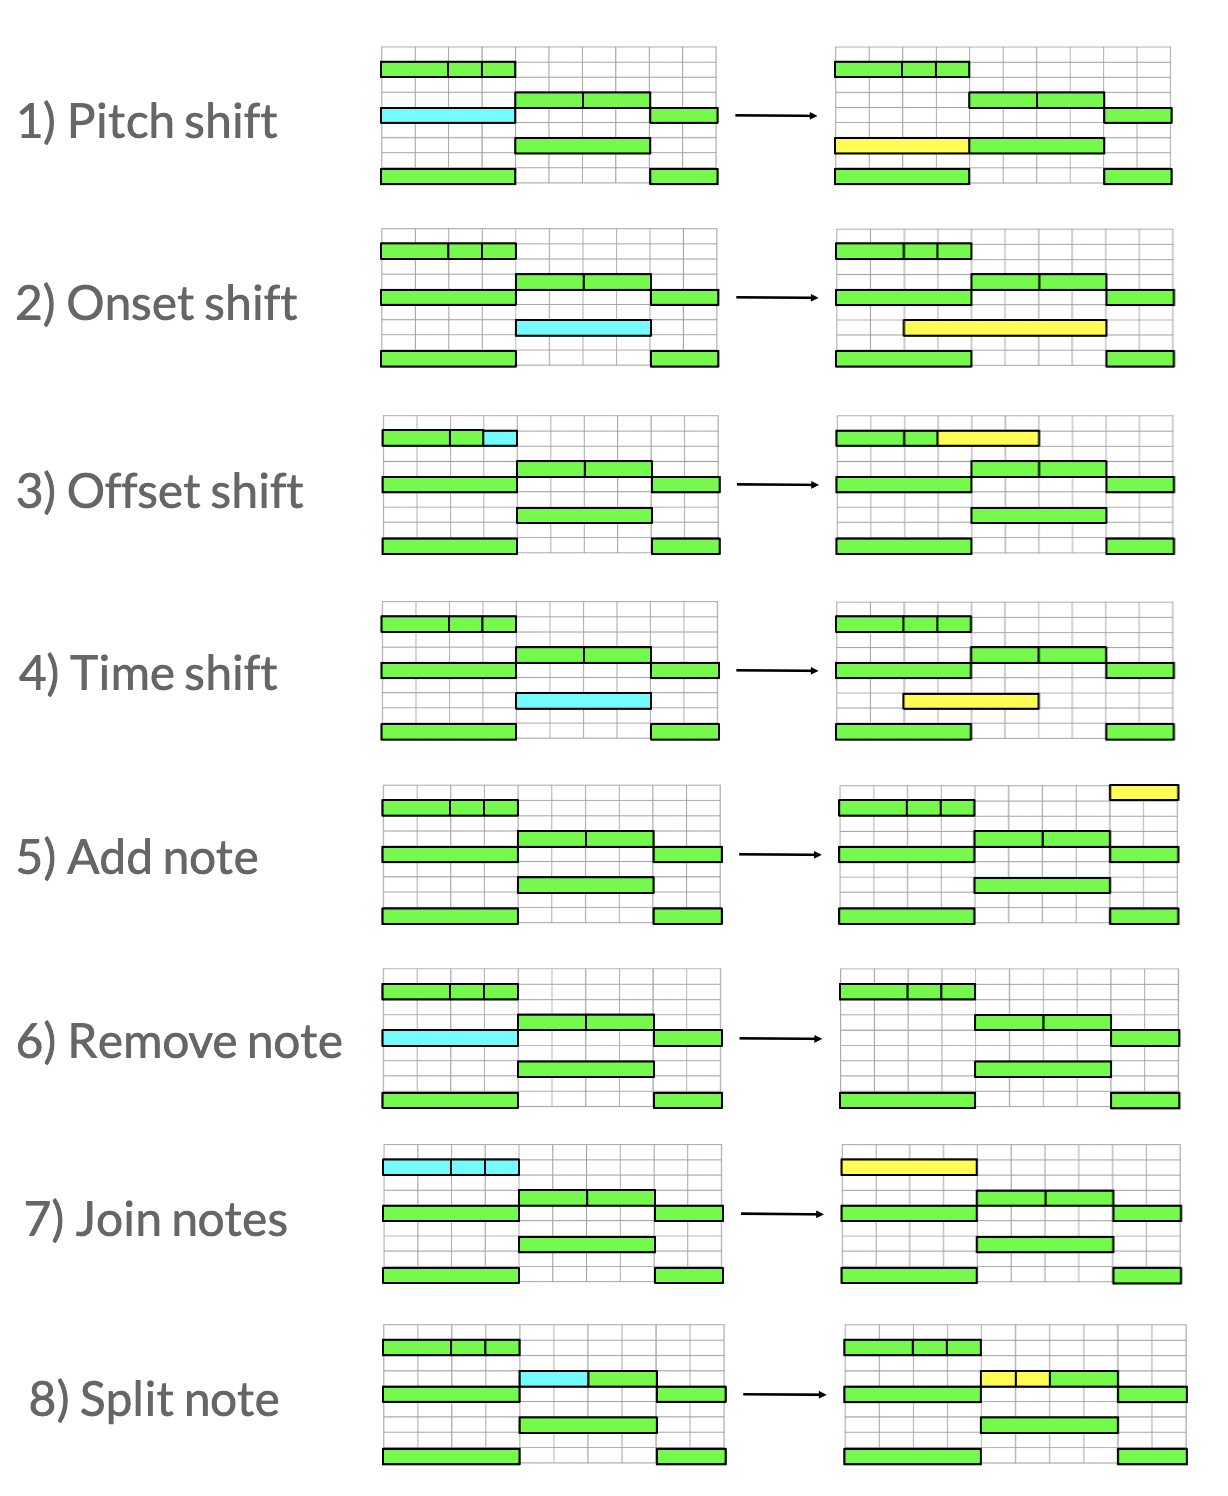
\includegraphics[width=1.0\textwidth]{source/figures/mdtk_degradations.png}
\caption[The degradations available in MDTK]{Illustrations for all the degradations currently available in MDTK}\label{fig:mdtk_degradations}
\end{figure}

We now briefly describe each of these degradations:

\begin{itemize}
\tightlist
\item
  Changes to pitch:

  \begin{enumerate}
  \def\labelenumi{\arabic{enumi}.}
  \tightlist
  \item
    \texttt{pitch\_shift}: changes the pitch of a random note. By
    default, the new pitch is chosen uniformly at random from all
    possible pitches (a minimum and maximum pitch can be given, and the
    valid range defaults to 21--108 inclusive). It can also be drawn
    from a weighted distribution of intervals around the original pitch,
    for example to emphasize octave errors from overtones. We also
    include a flag to force the new pitch to align with the pitch of
    some other note in the input, to reduce out-of-key shifts, if
    desired.
  \end{enumerate}
\item
  Changes to timing:

  \begin{itemize}
  \tightlist
  \item
    For all of these degradations, care is taken to ensure that the
    shifted note does not lie outside the input's initial time range. A
    minimum and maximum resulting duration can be specified, as well as
    a minimum and maximum shift amount. We also include flags to align
    some combination of the shifted note's onset or duration with those
    of other notes from the input, ensuring the note lies on some
    metrical grid, if desired.
  \end{itemize}

  \begin{enumerate}
  \def\labelenumi{\arabic{enumi}.}
  \setcounter{enumi}{1}
  \tightlist
  \item
    \texttt{onset\_shift}: changes the note's onset time (the time at
    which the note begins sounding), leaving its offset time (the time
    at which the note ends sounding) unchanged
  \item
    \texttt{offset\_shift}: changes the note's offset time, leaving its
    onset time unchanged
  \item
    \texttt{time\_shift}: changes the note's onset and offset times by
    the same amount, leaving its duration unchanged
  \end{enumerate}
\item
  Adding new notes or removing existing notes:

  \begin{enumerate}
  \def\labelenumi{\arabic{enumi}.}
  \setcounter{enumi}{4}
  \tightlist
  \item
    \texttt{add\_note}: introduces a new note, flags to align an added
    note's pitch, onset, or duration to those of existing notes are
    included.
  \item
    \texttt{remove\_note}: removes a random note from an input
  \end{enumerate}
\item
  Splitting/combining existing notes:

  \begin{enumerate}
  \def\labelenumi{\arabic{enumi}.}
  \setcounter{enumi}{6}
  \tightlist
  \item
    \texttt{split\_note}: cuts a random note into some number of
    consecutive notes of shorter duration (the first of which begins at
    the original note's onset time and the last of which ends at the
    original note's offset time). By default the note is split into two
    shorter notes, but this---as well as a minimum allowable duration
    for the resulting notes---can be set with a parameter.
  \item
    \texttt{join\_notes}: takes two or more consecutive notes at the
    same pitch (with a maximum allowable gap---set with a
    parameter---allowed between them), and joins them into a single note
    with onset time equal to that of the first note and offset time
    equal to that of the last.
  \end{enumerate}
\end{itemize}

\hypertarget{additional-tools-provided-by-mdtk}{%
\subsection{Additional tools provided by
MDTK}\label{additional-tools-provided-by-mdtk}}

MDTK also includes the \texttt{Degrader} class, which can be used to
degrade inputs dynamically. When instantiating a \texttt{Degrader}
object, the proportion of inputs that should remain undegraded is set
with a parameter (which can be 0). The probability of each degradation
being performed on the input (if it is to be degraded) can also be set
at this time. Then, each time \texttt{Degrader.degrade(input)} is
called, a randomly degraded version of the input is generated according
to the proportions set during object creation. The \texttt{Degrader}
class can be easily inserted into any model training procedure in order
to dynamically create new degraded inputs during each epoch, enabling
the model to be trained on a dataset which is essentially unlimited in
size.

Additional utility functions are provided to convert between MIDI format
and Pandas DataFrames (McKinney 2010) \& (The pandas development team
2021) holding the sequence of notes -- pandas DataFrames are a useful
data structure in Python to hold columnar data. The toolkit can also
handle data in the midi-like command format. An illustration of data
types is given in \Cref{fig:data_formats}.

\begin{figure}[htbp]
\centering
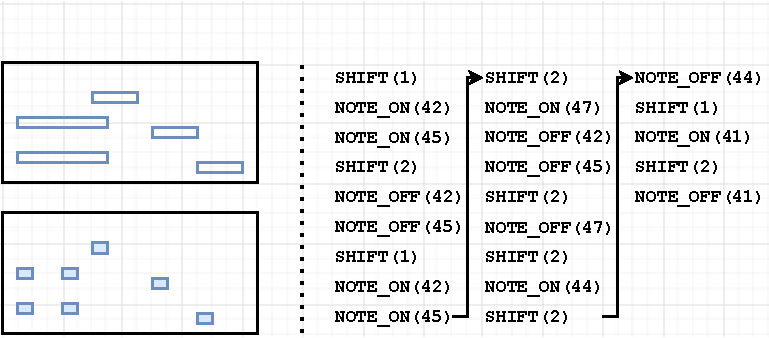
\includegraphics[width=1.0\textwidth]{source/figures/dataformats.pdf}
\caption[Different data formats handled by MDTK]{Data formats – On the left, a piano roll, on the right, the same data expressed as a sequence of commands. The piano roll has two parts - the first (shown above) indicates where notes are sounding, the second (shown below) shows where note onsets are happening.}\label{fig:data_formats}
\end{figure}

\hypertarget{an-experiment-illustrating-performance-gains-with-mdtk}{%
\section{An experiment illustrating performance gains with
MDTK}\label{an-experiment-illustrating-performance-gains-with-mdtk}}

\begin{figure}[htbp]
\centering

\includegraphics[width=1.0\textwidth]{source/figures/example.png}
\caption[Example MDTK degradation]{TODO: it’s not clear that we need this…leaving here for now. An example degradation performed by MDTK}\label{fig:mdtk_degradation_example}
\end{figure}

\hypertarget{evaluating-state-of-the-art-music-generating-models}{%
\chapter{Evaluating State-of-the-Art Music-generating
Models}\label{evaluating-state-of-the-art-music-generating-models}}

\begin{itemize}
\tightlist
\item[$\square$]
  If the main contribution is evaluating the long term structure, then
  ensure this is emphasized either in the title of this chapter or in
  the first lines
\end{itemize}

\hypertarget{comparative-analysis-using-new-and-existing-metrics}{%
\section{Comparative analysis using new and existing
metrics}\label{comparative-analysis-using-new-and-existing-metrics}}

\begin{itemize}
\tightlist
\item
  Use phrase and piece level metrics to evaluate state-of-the-art models
\item
  Compare and contrast, outlining the issues identified
  (e.g.~meandering, no high-level structure)
\end{itemize}

\hypertarget{strengths-and-shortcomings-of-existing-models}{%
\section{Strengths and shortcomings of existing
models}\label{strengths-and-shortcomings-of-existing-models}}

\hypertarget{avenues-for-improvement}{%
\section{Avenues for improvement}\label{avenues-for-improvement}}

\hypertarget{conclusion}{%
\chapter{Conclusion}\label{conclusion}}

\hypertarget{a-new-model}{%
\chapter{A New Model}\label{a-new-model}}

Potential ideas:

\begin{itemize}
\tightlist
\item
  An improved generative model for music

  \begin{itemize}
  \tightlist
  \item
    Training like BERT?
    \url{http://jalammar.github.io/illustrated-bert/}
  \item
    Using mdtk for data augmentation in training (negative examples?),
    making them more robust
  \item
    Alternative training objectives:

    \begin{itemize}
    \tightlist
    \item
      crossentropy slow and not musically informed
    \item
      can we use something akin to word error rate (this has been done
      for text)
    \end{itemize}
  \end{itemize}
\item
  Alternative ways to encode music: encoding chords and phrases in a
  low-rank continuous space

  \begin{itemize}
  \tightlist
  \item
    Have done some work on this with convnets and generating
    continuations

    \begin{itemize}
    \tightlist
    \item
      low rank was enforced by cross-product ing two vecs
    \end{itemize}
  \item
    Could investigate effect of different representations for music on
    performance
  \end{itemize}
\end{itemize}

\footnotesize
\singlespacing
\setlength{\parindent}{0in}

\hypertarget{references}{%
\chapter{References}\label{references}}

\ldots TODO\ldots{}

\begin{itemize}
\tightlist
\item[$\square$]
  check over using
  https://www.cl.cam.ac.uk/\textasciitilde ga384/bibfix.html
\item[$\square$]
  also check with https://github.com/yuchenlin/rebiber
\item[$\square$]
  Check all title casing correct (use curly braces around letters which
  should remain as they are). All titles should be in Title Case.
\end{itemize}

\hypertarget{refs}{}
\begin{CSLReferences}{1}{0}
\leavevmode\hypertarget{ref-antoniou_data_2018}{}%
Antoniou, A., Storkey, A. \& Edwards, H., 2018. Data {Augmentation}
{Generative} {Adversarial} {Networks}. Available at:
\url{https://openreview.net/forum?id=S1Auv-WRZ} {[}Accessed March 10,
2021{]}.

\leavevmode\hypertarget{ref-ariza_interrogator_2009}{}%
Ariza, C., 2009. The {Interrogator} as {Critic}: {The} {Turing} {Test}
and the {Evaluation} of {Generative} {Music} {Systems}. \emph{Computer
Music Journal}, 33(2), pp.48--70. Available at:
\url{https://www.jstor.org/stable/40301027} {[}Accessed January 22,
2021{]}.

\leavevmode\hypertarget{ref-briot_deep_2019}{}%
Briot, J.-P., Hadjeres, G. \& Pachet, F.-D., 2019. Deep {Learning}
{Techniques} for {Music} {Generation} -- {A} {Survey}.
\emph{arXiv:1709.01620 {[}cs{]}}. Available at:
\url{http://arxiv.org/abs/1709.01620} {[}Accessed January 22, 2021{]}.

\leavevmode\hypertarget{ref-cubuk_autoaugment_2019}{}%
Cubuk, E.D. et al., 2019. AutoAugment: Learning augmentation strategies
from data. In \emph{{IEEE} conference on computer vision and pattern
recognition, {CVPR} 2019, long beach, CA, USA, june 16-20, 2019}.
Computer Vision Foundation / {IEEE}, pp. 113--123. Available at:
\url{http://openaccess.thecvf.com/content_CVPR_2019/html/Cubuk_AutoAugment_Learning_Augmentation_Strategies_From_Data_CVPR_2019_paper.html}.

\leavevmode\hypertarget{ref-cuthbert_music21_2010}{}%
Cuthbert, M.S. \& Ariza, C., 2010. music21: {A} {Toolkit} for
{Computer}-{Aided} {Musicology} and {Symbolic} {Music} {Data}. In
\emph{Proceedings of the 11th {International} {Society} for {Music}
{Information} {Retrieval} {Conference}}. Available at:
\url{https://dspace.mit.edu/handle/1721.1/84963} {[}Accessed January 23,
2021{]}.

\leavevmode\hypertarget{ref-deng_imagenet_2009}{}%
Deng, J. et al., 2009. ImageNet: {A} large-scale hierarchical image
database. In \emph{2009 {IEEE} computer society conference on computer
vision and pattern recognition {(CVPR} 2009), 20-25 june 2009, miami,
florida, {USA}}. {IEEE} Computer Society, pp. 248--255. Available at:
\url{https://doi.org/10.1109/CVPR.2009.5206848}.

\leavevmode\hypertarget{ref-dhariwal_jukebox_2020}{}%
Dhariwal, P. et al., 2020. Jukebox. \emph{OpenAI}. Available at:
\url{https://openai.com/blog/jukebox/} {[}Accessed February 19, 2021{]}.

\leavevmode\hypertarget{ref-dong_muspy_2020}{}%
Dong, H.-W. et al., 2020. {MusPy}: {A} {Toolkit} for {Symbolic} {Music}
{Generation}. In \emph{Proceedings of the 21st {International} {Society}
for {Music} {Information} {Retrieval} {Conference}}. Montreal, Canada.
Available at:
\url{https://program.ismir2020.net/static/final_papers/187.pdf}
{[}Accessed January 26, 2021{]}.

\leavevmode\hypertarget{ref-giraud_computational_2016}{}%
Giraud, M., Groult, R. \& Levé, F., 2016. Computational {Analysis} of
{Musical} {Form}. In D. Meredith, ed. \emph{Computational {Music}
{Analysis}}. Cham: Springer International Publishing, pp. 113--136.
Available at: \url{https://doi.org/10.1007/978-3-319-25931-4_5}
{[}Accessed February 21, 2021{]}.

\leavevmode\hypertarget{ref-haddow_wmt_2020}{}%
Haddow, B., 2020. {EMNLP} 2020 {Fifth} {Conference} on {Machine}
{Translation} ({WMT20}). \emph{2020 Fifth Conference on Machine
Translation (WMT20)}. Available at: \url{http://www.statmt.org/wmt20/}
{[}Accessed January 23, 2021{]}.

\leavevmode\hypertarget{ref-hollings_ada_2018}{}%
Hollings, C., Martin, U. \& Rice, A.C., 2018. \emph{Ada {Lovelace}:
{The} {Making} of a {Computer} {Scientist}}, Oxford: Bodleian Library.

\leavevmode\hypertarget{ref-huang_music_2019}{}%
Huang, C.-Z.A. et al., 2019. Music transformer: Generating music with
long-term structure. In \emph{7th international conference on learning
representations, {ICLR} 2019, new orleans, LA, USA, may 6-9, 2019}.
OpenReview.net. Available at:
\url{https://openreview.net/forum?id=rJe4ShAcF7}.

\leavevmode\hypertarget{ref-lewis_bart_2020}{}%
Lewis, M. et al., 2020. {BART}: Denoising sequence-to-sequence
pre-training for natural language generation, translation, and
comprehension. In \emph{Proceedings of the 58th annual meeting of the
association for computational linguistics}. Online: Association for
Computational Linguistics, pp. 7871--7880. Available at:
\url{https://www.aclweb.org/anthology/2020.acl-main.703}.

\leavevmode\hypertarget{ref-lu_speller100_2021}{}%
Lu, J., Long, J. \& Majumder, R., 2021. Speller100 expands spelling
correction technology to 100+ languages. \emph{Microsoft Research}.
Available at:
\url{https://www.microsoft.com/en-us/research/blog/speller100-zero-shot-spelling-correction-at-scale-for-100-plus-languages/}
{[}Accessed March 7, 2021{]}.

\leavevmode\hypertarget{ref-marsden_music_2016}{}%
Marsden, A., 2016. Music {Analysis} by {Computer}: {Ontology} and
{Epistemology}. In D. Meredith, ed. \emph{Computational {Music}
{Analysis}}. Cham: Springer International Publishing, pp. 3--28.
Available at: \url{https://doi.org/10.1007/978-3-319-25931-4_1}
{[}Accessed February 17, 2021{]}.

\leavevmode\hypertarget{ref-mckinney_data_2010}{}%
McKinney, W., 2010. Data {Structures} for {Statistical} {Computing} in
{Python}. In Austin, Texas, pp. 56--61. Available at:
\url{https://conference.scipy.org/proceedings/scipy2010/mckinney.html}
{[}Accessed March 10, 2021{]}.

\leavevmode\hypertarget{ref-mcleod_midi_2020}{}%
McLeod, A., Owers, J. \& Yoshii, K., 2020. The {MIDI} {Degradation}
{Toolkit}: {Symbolic} {Music} {Augmentation} and {Correction}. In
\emph{Proceedings of the 21st {International} {Society} for {Music}
{Information} {Retrieval} {Conference}}. Montreal, Canada. Available at:
\url{https://program.ismir2020.net/static/final_papers/182.pdf}
{[}Accessed January 26, 2021{]}.

\leavevmode\hypertarget{ref-payne_musenet_2019}{}%
Payne, C., 2019. {MuseNet}. \emph{OpenAI}. Available at:
\url{https://openai.com/blog/musenet/} {[}Accessed January 23, 2021{]}.

\leavevmode\hypertarget{ref-van_rossum_python_1995}{}%
Rossum, G. van, 1995. Python tutorial. Available at:
\url{https://ir.cwi.nl/pub/5007} {[}Accessed February 21, 2021{]}.

\leavevmode\hypertarget{ref-salamon_deep_2017}{}%
Salamon, J. \& Bello, J.P., 2017. Deep {Convolutional} {Neural}
{Networks} and {Data} {Augmentation} for {Environmental} {Sound}
{Classification}. \emph{IEEE Signal Processing Letters}, 24(3),
pp.279--283.

\leavevmode\hypertarget{ref-sturm_ai_2020}{}%
Sturm, B., 2020. {AI} {Music} {Generation} {Challenge} 2020. \emph{The
2020 Joint Conference on AI Music Creativity}. Available at:
\url{https://boblsturm.github.io/aimusic2020/} {[}Accessed January 22,
2021{]}.

\leavevmode\hypertarget{ref-sturm_benchmarking_2017}{}%
Sturm, B.L.T., 2017. Benchmarking {``music generation systems?''}
\emph{Folk the Algorithms}. Available at:
\url{https://highnoongmt.wordpress.com/2017/03/19/benchmarking-music-generation-systems/}
{[}Accessed February 18, 2021{]}.

\leavevmode\hypertarget{ref-pandas_software_2021}{}%
The pandas development team, 2021. Pandas-dev/pandas: {Pandas} 1.2.3.
Available at: \url{https://zenodo.org/record/4572994\#.YEhrWV37Rb8}
{[}Accessed March 10, 2021{]}.

\leavevmode\hypertarget{ref-theis_note_2016}{}%
Theis, L., Oord, A. van den \& Bethge, M., 2016. A note on the
evaluation of generative models. In Y. Bengio \& Y. LeCun, eds.
\emph{4th international conference on learning representations, {ICLR}
2016, san juan, puerto rico, may 2-4, 2016, conference track
proceedings}. Available at: \url{http://arxiv.org/abs/1511.01844}.

\end{CSLReferences}

\end{document}
% ### END TEMPLATE.TEX ###
